\chapter{Results}

\section{Bulk droplets}

\begin{figure}
\centering
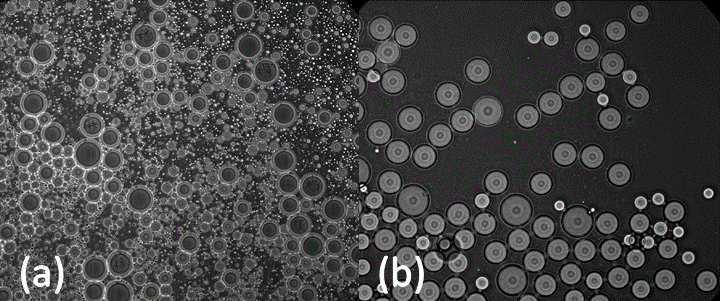
\includegraphics[width=\linewidth]{graphics/2025_09_28_droplets_fig3.png}
\caption{\textbf{Comparison of bulk droplets and on-chip droplets reveals broad size distribution in bulk droplets}}
\label{fig:results_droplet_bulk_vs_chip}
\end{figure}

\section{On-chip doplet production}

\section{Identifying producer-target pair}
After choosing our antibiotic producing strain, we used the well established halo-assay method to screen a collection of possible target strains, selected based on similar growth rate and easy culture conditions. We observe inhibition for several of the possible targets. Based on these results, we chose a \textit{Staphylococcus aureus} strain due to the large inhibition zone combined with its clinical significance. We ...

\begin{figure}
\centering
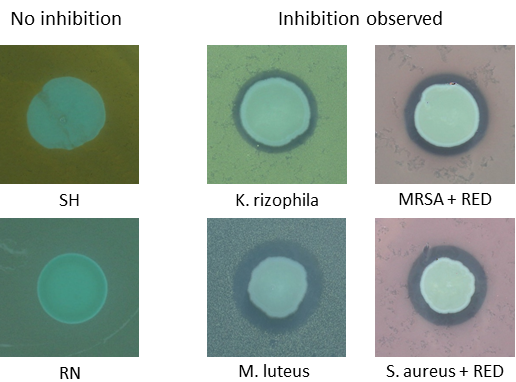
\includegraphics[width=\linewidth]{graphics/2025_09_28_droplets_fig4.png}
\caption{\textbf{Halo assay for library of target strains identifies \textit{S. aureus} as potential target}}
\label{fig:results_sensitive_screening}
\end{figure}

\section{B. subtilis stressed in droplets}
After establishing the technical platform, we can incubate droplets for long periods of time and can monitor them under the microscope during these incubation periods.

\begin{figure}
\centering
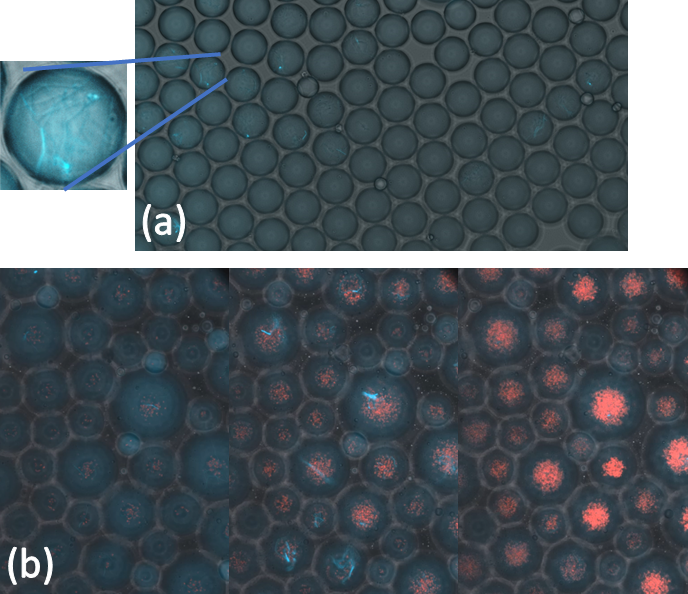
\includegraphics[width=\linewidth]{graphics/2025_09_28_droplets_fig5.png}
\caption{\textbf{On-chip droplets are stable after long-term incubation and allow bacterial growth}}
\label{fig:results_incubation_subtilis}
\end{figure}

\section{Liquid vs. droplet comparison}
To understand if \textit{B. subtilis} disappears only in droplets or also in liquid, we performed a liquid-droplet comparison assay with separate cultures of B. subtilis and S. aureus. After incubation for 21h with high inoculation densities, we see that both liquid cultures exhibted growth while in droplets only the \textit{S. aureus} culture exhibits growth. The \textit{B. subtilis} culture in droplets seems to not support growth of bacteria.

\begin{figure}
\centering
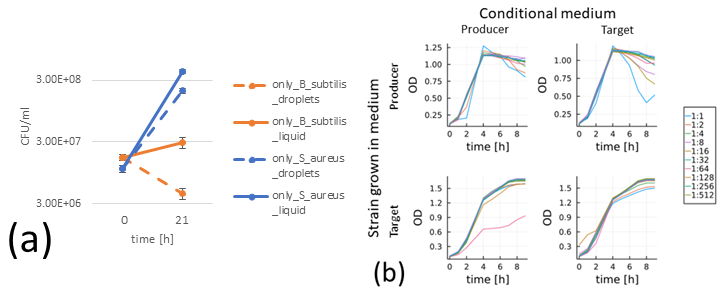
\includegraphics[width=\linewidth]{graphics/2025_09_28_droplets_fig6.png}
\caption{\textbf{\textit{B. subtilis} fails to grow in droplets and does not kill in liquid}}
\label{fig:results_liquid_vs_drop_supernatant}
\end{figure}

\section{Lack of antibiotic production in liquid}
Using an established conditional medium assay, we created a dilution series of the medium in which the producer previously grew. 